%!TEX root = thesis.tex
\chapter{Related work}
\label{chap:rw}

\section{CityJSON}
\label{sec:cityjsonexplained}

CityJSON \citep{cityjsonspecs} is an encoding for storing digital twins, containing geometries and attributes of real world features such as buildings, terrains, roads, and waterbodies.
It is based on the data model of CityGML \citep{citygml}, but uses \ac{json} as encoding for it rather than \ac{gml} which poses advantages in file compactness and ease of use.
The file format has four main characteristics that can be exploited for compression purposes: the \ac{json} encoding, geometries, attributes, and textures.
As mentioned in Section~\ref{sec:datacompression}, prior knowledge on the input data allows for more suitable compression techniques to be chosen.
Furthermore, the explanation helps in understanding the difference with other file formats that are introduced in Sections~\ref{sec:b3dm} and~\ref{sec:i3s}.

The \ac{json} format is easy for humans to read, while at the same time relatively lightweight (in comparison to for example \ac{gml}) \citep{json}.
In its specification several data types are defined: boolean values, numbers, strings, arrays (ordered lists of elements), and objects (containing key-value pairs).
These data types can be combined and nested \citep{ledoux2019cityjson}.
In Listing~\ref{ls:cj2} it is shown how this looks like with example snippet of a CityJSON dataset.
However, the readability comes at the cost of verbosity.
This is exemplified by the binary JSON-like format \ac{cbor} which is introduced in Section~\ref{sec:cbor}.

A CityJSON file is a \ac{json} object contains 4 mandatory keys:
\begin{enumerate}
\item \texttt{"type"} (which is always of value \texttt{"CityJSON"})
\item \texttt{"version"}
\item \texttt{"CityObjects"} (a \ac{json} object containing objects that represent geographical features)
\item \texttt{"vertices"} (an array containing the coordinates of all vertices)
\end{enumerate}

A feature in CityJSON is called a city object and can be of a variety of types (shown in Table~\ref{tab:cityobjects}) as derived from CityGML's data model \citep{ledoux2019cityjson}.
A city object is not limited to these types, as extensions can add others.
A 2nd-level city object can be a child of a 1st-level city object parent, and thus linked together in this way.





It always has a \texttt{"geometry"} key which is an array containing more than 0 geometry objects, which can represent several \ac{lod}s.
A geometry object in turn can be of several types of 3D geometric primitives.
The vertex coordinates of a 3D model are stored in one array as shown in the above list, but the connectivity information is stored in geometry objects.
Here, references to vertices are stored.
This is inspired on the Wavefront OBJ \citep{Reddy} format, and these parts are depicted in the green in listings~\ref{ls:cj2}, and ~\ref{ls:cj3}.
Optionally, a city object can have an "attributes" object as member.
Here all attributes can be stored as defined in CityGML's data model, with which extension is possible as well \citep{ledoux2019cityjson, cityjsonspecs}.

%These elements are marked with the red rectangles in listings~\ref{ls:cj1} and ~\ref{ls:cj2}.

In addition, there are optional keys for extensions, metadata, coordinate transform, appearance, and geometry-templates. 
Metadata can contain for example the geographical extent of the data, and coordinate transform gives the option to define a coordinate offset, which enables compression through the conversion of coordinates to integers and moving the origin to (0, 0, 0) \citep{ledoux2019cityjson, cityjsonspecs}.
This actually is a form of quantisation (Section~\ref{theoryquantisation}).
The basic structure of a CityJSON file is shown in listing~\ref{ls:cj1}, including \texttt{"metadata"} and \texttt{"transform"}.

Lastly, it can contain materials, textures, and semantic surfaces belonging to city objects.
These are respectively stored following the X3D specifications and with additional COLLADA files \citep{ledoux2019cityjson, cityjsonspecs}.
This is however out of the thesis scope (see~\ref{sec:scope}).

\begin{table}
 \begin{tabular}{ |l|l| } 
 \hline
  1st-level city objects & 2nd-level city objects\\
 \hline \hline
      \multirow{2}{45mm}{Building}&BuildingPart\\
    &BuildingInstallation\\
\hline
      \multirow{3}{45mm}{Bridge}&BridgePart\\
    &BridgeInstallation\\
    &BridgeConstructionElement\\
\hline
\multirow{10}{45mm}{CityObjectGroup\\CityFurniture\\GenericCityObject\\LandUse\\PlantCover\\Railway\\Road\\SolitaryVegetationObject\\TINRelief\\TransportSquare} 
      &\\
      & \\
      & \\
      &\\
      & \\
      &\\
      & \\
      & \\
      &\\
      & \\
\hline
      \multirow{2}{45mm}{Tunnel}&TunnelPart\\
    &TunnelInstallation\\
\hline
WaterBody & \\
\hline
\end{tabular}
\caption{Types of city objects (features) that CityJSON natively supports (from \citet{ledoux2019cityjson}}
\label{tab:cityobjects}
\end{table}

\clearpage

\begin{scriptsize}
\hspace{-1.6cm}\begin{minipage}[c]{0.45\linewidth}

\lstdefinestyle{base}{
backgroundcolor=\color{lichtgrijs}, 
  moredelim=**[is][\color{orange}]{@}{@},
}

\begin{lstlisting}[frame=single,style=base,caption={Snippet of CityJSON structure, with mandatory members in orange}, label=ls:cj1]
{
    @"type": "CityJSON",@	
    @"version": "1.0",@	
    @"CityObjects": {..},@	
    @"vertices": {..},@	
    "metadata": {
        "geographicalExtent": [	
            84616.468,	
            447422.999,	
            -0.47,	
            85140.839,	
            447750.636,	
            13.8	
            ],	
        "referenceSystem": "urn:ogc:def:crs:EPSG::7415"	
        },	
    "transform": {	
        "scale": [	
            0.001,	
            0.001,	
            0.001	
            ].	
        "translate": [	
            84616.468,	
            447422.999,	
            -0.47		
    }
}
\end{lstlisting}


\end{minipage}
\hspace{0.2cm}
\begin{minipage}[c]{0.42\linewidth}

\lstdefinestyle{base}{
backgroundcolor=\color{lichtgrijs}, 
  emptylines=1,
  breaklines=true,
basicstyle=\ttfamily\color{black},
  moredelim=**[is][\color{orange}]{@}{@},
moredelim=**[is][\color{Green}]{|}{|},
}

\begin{lstlisting}[frame=single,style=base,caption={Snippet of basic structure of CityObjects. Attributes in orange, geometries in green}, label=ls:cj2]
{
    "type": "CityJSON",
    "version": "1.0",
     "CityObjects": {
        "b0a8da4cc-2d2a-11e6-9a38": {
            @"type": "BuildingPart",@	
            @"attributes": {@	
            @"creationdate": "2014-07-09",@	
                @"terminationdate": "",@	
                @"function": "garage"@	
                @},@	
                |"geometry": [|	
                |{|	
                    |"type": "Solid",|	
                    |"boundaries": [|	
                        |[|	
                            |[|	
                                |[|	
                                    |[0, 1, 2],|	
                                    |[1, 2, 3],|	
                                    |[1, 3, 4],|	
                                    |[0, 1, 4]|	
                                |]|	
                            |]|	
                        |]]|	
                    |},|	
                    |"lod": 2,|	
                |},|	
            "parents": ["b0a8da4cc-2d2a-11e6-9a39"]
            },
        "b1105d28c-00ba-11e6-b420": {..},
        "b1126a169-00ba-11e6-b420" {..}
    },
    |"vertices": [..]|
}
\end{lstlisting}


\end{minipage}
\hspace{0.2cm}
\begin{minipage}[c]{0.30\linewidth}

\begin{lstlisting}[frame=single,style=base,caption={Snippet of vertex array of CityJSON, highlighted in green}, label=ls:cj3]
{
    "type": "CityJSON",
    "version": "1.0",
    "metadata": {..},
    "CityObjects": {..},
     |"vertices": [|	
          |85012.343,|	
          |447455.577,|	
          |-0.27|	
          |],|	
          |[|	
          |85010.804,|	
          |447448.808,|	
          |-0.27|	
          |],|	
          |[|	
          |85013.832,|	
          |447447.447,|
          |-0.27|	
          |],|	
          ...
}
\end{lstlisting}

\end{minipage}
\end{scriptsize}


\section{Draco}
\label{rwdraco}

Draco, an open-source library by Google for compression and decompression of geometric meshes \citep{draco}, can be used to compress the geometrical part of the CityJSON structure.
Generally, it works with the Edgebreaker algorithm (which is explained in Section~\ref{sec:theoryedgebreaker}), their own sequential connectivity method (Subsection~\ref{sec:seqconnectivity}), parallelogram prediction (Subsection~\ref{sec:parallelogram}), and the quantisation of coordinates (Subsection~\ref{theoryquantisation}).
It can compress both 3D geometrical meshes and point clouds, but only the former is relevant for this application.
On average, it compresses meshes (that are in Wavefront OBJ format) to about 2 percent of their original file size \citep{dracoperformance}.
It has encoders and decoders written in C++ and JavaScript (and exclusively a decoder in WebAssembly), enabling it to be suitable for both offline (in this case preparation of compressed CityJSON files) and online (decoding the compressed geometries in the browser) purposes.\\

Not just the savings on file storage itself are beneficial, but since files are transferred over the web for browser use, time is saved as the data is in a slimmer format.
The network speed can form a bottleneck, and it is exemplified by Cesium that using Draco can potentially improve the rendering speed as it is decoded asynchronously, meaning that parts are already rendered while the complete dataset is still being downloaded \citep{cesiumdraco}.


There are three main configurations that can be set when encoding a mesh.
First, there is the compression level parameter which goes from 0 to 10.
Based on this parameter, different compression features that the library encompasses are used, with 10 giving the most compressed result but at the same time having the worst decompression time.
Second, a parameter that specifies the amount of bits to which the input values should be quantised can be chosen (which would make the compression lossy if used---see Section~\ref{theoryquantisation}), and lastly, there is the option to retain the separation between objects \cite{dracoperformance}.


Draco compressed meshes are stored in their native .drc binary format.
The format generally consists of four parts: a header, metadata (object id for example), connectivity data, and attributes, as shown on Figure~\ref{fig:draco_format}.


\begin{figure}[h!]
    \centering
    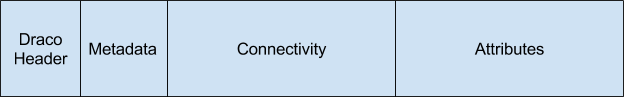
\includegraphics[scale=0.5]{figs/related_work/draco_format.png}
    \caption{The general structure of the Draco file format (.drc). Figure taken from \citet{dracospec}}
    \label{fig:draco_format}
\end{figure}


%\section{Text compression}
%Besides the geometry of CityJSON files, its semantics that are repesented as text can be compressed as well. 

\section{glTF}
\label{sec:gltf}
\ac{gltf} is a file format that is designed for efficient loading of 3D graphics and their dissemination over the internet \citep{KhronosGroup2019}. 
It is formatted in \ac{json} and keeps file sizes small, can be processed fastly and is an extensible format.
The elements that it contains conceptually have a hierarchical relationship as shown in Figure~\ref{fig:gltf}.
Roughly explained, a scene is one model, and a file can contain multiple ones.
A scene in turn contains nodes (which are features---for example a building).
These do not have a specified \ac{crs}, but can have their own translation, rotation, and scale properties, similar to CityJSON's \texttt{"transform"} (see Section~\ref{sec:cityjsonexplained}.
Their geometries are stored in a combination of meshes, buffers, bufferViews, and accessors, and it is possible to include skins, animations, cameras, materials, and textures.
Moreover, it is possible to include for example buffer geometries and textures in binary format.

\begin{figure}[h!]
    \centering
    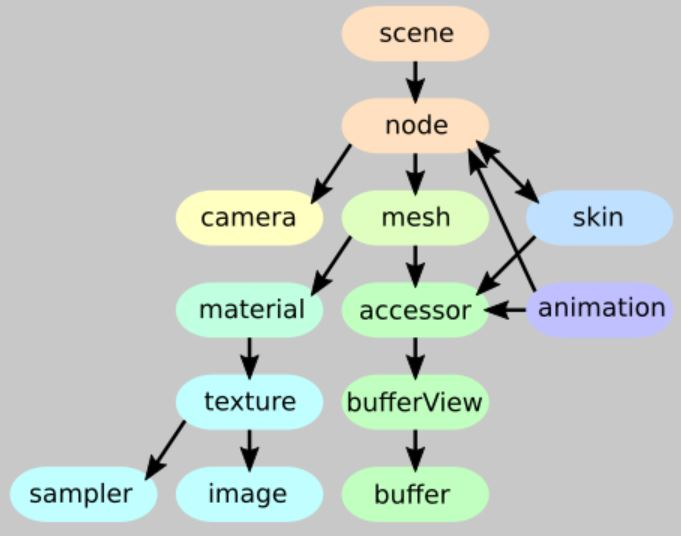
\includegraphics[scale=0.5]{figs/related_work/gltf.jpg}
    \caption{The conceptual structure of the \ac{gltf} format (cropped from \citet{KhronosGroup2019})}
    \label{fig:gltf}
\end{figure}

\section{Cesium 3D Tiles}
\label{sec:3dtiles}
Despite this part being out of scope for this thesis (as stated in the introduction), it is still important to notice its existence as it can make a contribution to the efficient streaming of 3D geoinformation.
Besides that, it is implemented by the \ac{b3dm} format (see Section~\ref{sec:b3dm}), which is an alternative to CityJSON for web visualisation.

Created for the sharing, visualisation, and analysis of 3D geoinformation, the 3D Tiles specification \citep{3dtiles} is a \ac{json} object in which the data is separated into tiles.
Every tile is described by a bounding volume and the tiles are organised into a tree, which could be a quadtree, octree, k-d tree, or grid.
Tiles can have children, creating a hierarchical structure with which different LoD can be represented.
The tile parent would contain the 3D model in a low LoD, and every child would contain either more details that can be rendered when needed, or again a full 3D model but with a higher LoD \citep{Cesium2020}.

Its implementation can thus benefit the streaming of massive datasets as it allows the loading of smaller parts (tiles) as they are needed, e.g. when they are zoomed into, and in the LoD that they are wanted.
In Section~\ref{sec:b3dm} an implementation of 3D Tiles is explained, giving more details about the structure.


\subsection{Batched 3D Model}
\label{sec:b3dm}
b3dm is a binary file format that can store heterogeneous 3D models and incorporates the 3D Tiles specification \citep{b3dm}.
It roughly consists of three parts: a feature table, batch table, and \ac{gltf} geometry.
In the specification a feature is a 3D model and the feature table can thus be seen as a collection of tiles.
Every feature may have a position property indicating the coordinates of its centre.

In the batch table the properties of the contents of features are contained.
These properties are stored in \ac{json} format, but in a different fashion than CityJSON's CityObjects. 
It is an array value with the name of the property as key, with the array containing values for the ordered objects of the feature.
This means that if there is an n amount of objects, the array for a property will contain n elements.
An example is as follows:

\blockquote{"height" : [10.0, 20.0, 15.0]}

Alternatively, the properties can be stored in a binary body to which a reference is placed within the aforementioned JSON structure.
Since this way of storing attributes is inefficient when there are properties that only apply to a subset of objects (for example "amount of leafs" for trees, which buildings would not have), it is possible to define object types which have their own set of property names.

Lastly, the geometries of the objects from all features are stored as \ac{gltf}, which allows for the use of Draco compression as well since it can be embedded therein.

The format therefore is similar to the aimed end-result of this thesis, with the additional benefit of having the option to structure the data into tiles.
On the contrary, it lacks the benefits of the CityGML data structure, the tools that exist for CityJSON, and (further) compression of attributes \citep{b3dm}.

\section{Esri I3S}
\label{sec:i3s}
\ac{i3s} \citep{i3sspecsmain} is an open file format by Esri.
The scene layer that it encodes in turn contains large volume heterogeneous geographic data (\eg\ 3D objects, point clouds, and buildings). 
It is formatted in JSON and specifically designed for the efficient streaming of massive 3D datasets. 
Similarly to CityJSON, Scene Layers encompass the geometry, texture, and attributes of features. 
Features are grouped into nodes with the nodes forming a regular or irregular tree by their bounding sphere (or oriented bounding box), akin to respectively a quadtree or an R-tree.
Parent nodes in a tree contain the features with a lower LoD.
Because of this structure, specific nodes can be found faster and loaded more efficiently as well as simpler representations of geometries can be shown when they are looked at from afar \citep{i3sspecs, i3sspecsmain}.

A node in itself does not contain complete features, but rather IDs which point to geometry buffers (encoded with Draco), textures, and attributes.
The standard allows any geodetic coordinate reference system to be used, with the node having the same \ac{crs} as the vertices that it encompasses.
The vertex position are stored with the centre of the node's bounding area as offset, allowing for compression and easier visualisation in for example three.js.
LoD are not the same in I3S as in CityJSON---it uses thinning, clustering, and generalisation of 3D objects or meshes, as well as the downsampling of textures.
The to-be visualised LoD (thus which leaf of the tree is chosen by the viewer) is determined by screen size, resolution, bandwith, and memory \citep{i3sspecsmain, i3sspecs}.




\section{Binary JSON}
Binary file formats can be more concise and processed (reading or writing) faster, as explained in Section~\ref{sec:binary}.
It is therefore relevant for the improvement of CityJSON's efficiency.
Additionally, it can be beneficial to store binary data in JSON format, such as encryption keys or graphics like Draco geometries (see~\ref{rwdraco}).
JSON natively does not allow for this and requires such data to be encoded in Base64 format.
This is a family of binary-to-text encoding schemes that is utilised when binary data needs to be stored, while working with media that are created to handle ASCII rather than binary data \citep{cborurl}.
The downside of this is that a string in Base64 encoding can be 33\% larger than its binary form \citep{Mozilla2020}.

There are several different binary formats that encode data in a JSON-like manner.
In a \ac{json} library for C++ by \citet{nlohmann}, the following ones are implemented: \ac{bson}, MessagePack, \ac{ubjson}, and \ac{cbor}.
I have chosen to use \ac{cbor} for the reasons below, as derived from a comparison with \ac{cbor} from \citet{cborspecs}, but this does not necessarily mean it is the best-performing option for the use cases of this thesis.
\ac{bson} is specifically developed for MongoDB \citep{MongoDB2020}.
This means that it is adapted for that purpose and this could make it less efficient for other purposes.
It does have the possibility for updating values, but this comes at the cost of less concise storage.
MessagePack is similar to \ac{cbor}, but has caveats that have to do with backwards compatibility and there is not much space for extension of the specification anymore.
\ac{ubjson} exactly mimics the \ac{json} data model, which means that it can not store binary values.
However, this functionality is necessary for storing Draco geometries within a CityJSON-like (compressed) file.





\subsection{CBOR}
\label{sec:cbor}
\ac{cbor} has two clear purposes that were stated prior to its development, which are storing binary strings into a JSON-like format and compression of data \citep{cborurl}.
Like \ac{json}, it follows a key-value structure. 
Roughly explained, every data item starts with an initial byte the contains information about the major type of the item and supplementary information.
The major type can be one of the following \citep{cborspecs}:
\begin{itemize}
\item Unsigned integer
\item Negative integer
\item Byte string
\item Text string
\item Array
\item Map (JSON-style object)
\item Optional semantic tagging of other types (such as date/time string, URI, base64)
\item Floating-point number
\end{itemize}

When reading the data, knowing the type and length of a value increases the performance as mentioned in Section~\ref{sec:binary}.
